\subsection*{Level 1}
Since the plant have a transfer function as,
\begin{equation}
  G_o(s)=\frac{25.15}{s+2.157}
\end{equation}
and that an $A_m(s)$ of same order as the plant should be chosen, the
following functions was used,
\begin{align*}
    A_m(s)=s+\omega_1 \\
    A_o(s)=s+\omega_2
\end{align*}
with
\begin{align*}
    \omega_1 = 10 \\
    \omega_2 = 5.
\end{align*}
These values gives the plot seen in figure \ref{fig:sens31org}.
\begin{figure}[H]
  \centering
  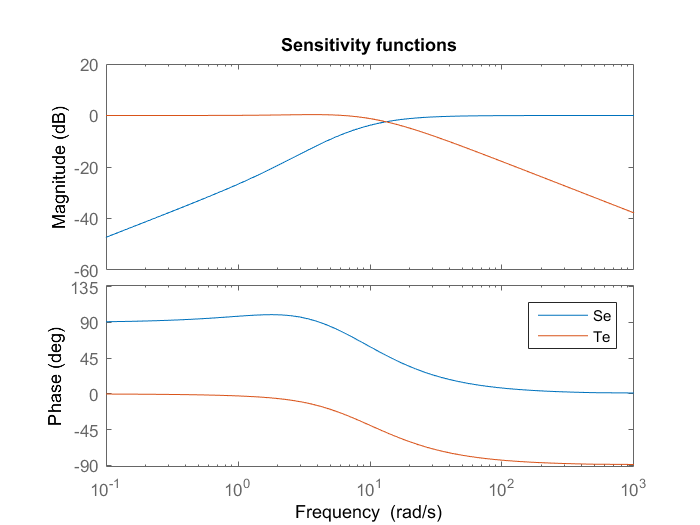
\includegraphics[width=0.45\linewidth]{plot31org.png}
  \caption{The sensitivity and conmplementary sensitivity function.}
  \label{fig:sens31org}
\end{figure}
When the poles for $A_0(s)$ is increased to five times $A_m(s)$ the
results in figure \ref{fig:sens31fast} is obtained. 
\begin{figure}[H]
    \centering
    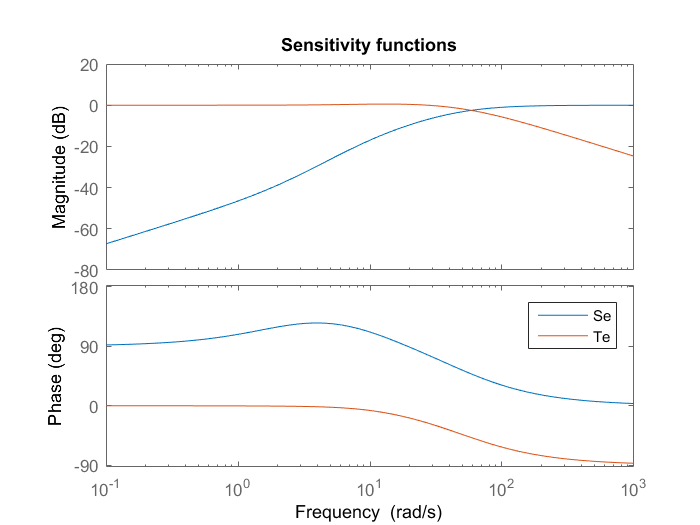
\includegraphics[width=0.45\linewidth]{plot31fast.png}
    \caption{$S_e$ and $T_e$ with five times faster $A_o(s)$ poles.}
    \label{fig:sens31fast}
\end{figure}
From the plots we can see that there is a possibility to adjust the
system to be less sensitive to noise and disturbances from either the
sensor or the plant. This means that if there is a good plant model,
there is less sensitivity to sensor noise.
